\section{Zielsetzung}
\label{sec:Zielsetzung}
In diesem Versuch wird die Funktionsweise eines Diodenlaser betrachtet und
mithilfe dieses sollen verschiedene Resonanzlinien von Rubidium aufgenommen werden.

\section{Theorie}
\label{sec:Theorie}

\subsection{Hintergrund}
Vor der Entwicklung des Diodenlasers wurden Laser

\subsection{Aufbau und Funktionsweise}
Der allgemeine Aufbau eines Lasers besteht aus einer Pumpquelle, ein Lasermedium
und einem Resonator, wie in Abbildung \ref{fig:laser} abgebildet. Dieser Aufbau
wird auch bei einem Diodenlaser verwendet.
\begin{figure}[htb]
  \centering
  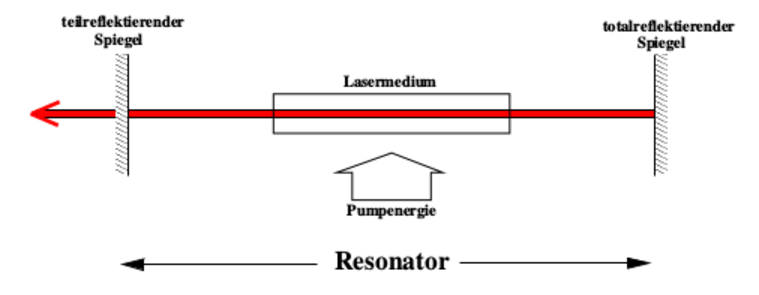
\includegraphics[width=0.8\textwidth]{images/V61.pdf}
  \caption{Schematische Darstellung der allgemeinen Laserkomponenten \cite{anleitung2}.}
  \label{fig:laser}
\end{figure}
Die Aufgaben der einzelen Bestandtteile werden in einem Diode-Chip und einen
äußeren Resonator zusammengefasst.

\subsubsection{Dioden-Chip}
Der Grundbaustein eines Diodenlasers besteht aus dem Dioden-Chip. Wie in
Abbildung \ref{fig:chip} zu sehen, besteht der quaderförmige Chip aus einer
Halbleiter-Heterostuktur (Abbildung \ref{fig:struktur}), welche ebenso als
optischer Wellenleiter dient. Um
einen Laserlicht erhalten zu können soll es in einer der Lagen zur Rekombination
eines Elektron-Loch-Paares kommen. Dazu wird nun der Aufbau dieser Diode näher
beleuchtet.

\begin{figure}
  \begin{subfigure}[c]{0.5\textwidth}
    \centering
    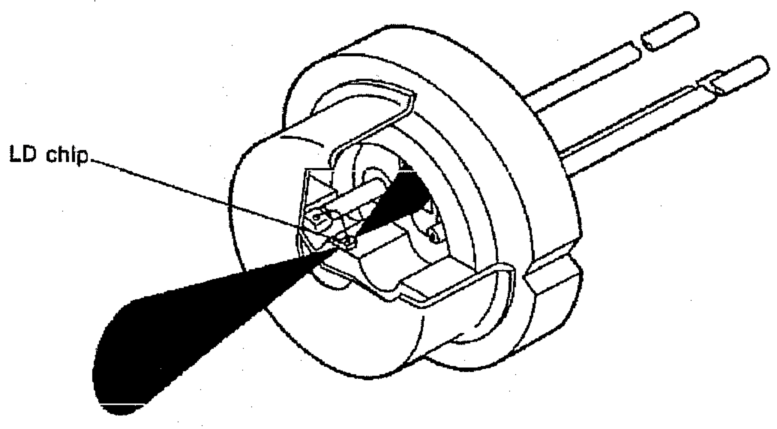
\includegraphics[width=\textwidth]{images/Diodenl.pdf}
    \subcaption{Darstellung des Lasers.}
    \label{fig:chip}
  \end{subfigure}
  \begin{subfigure}[c]{0.5\textwidth}
    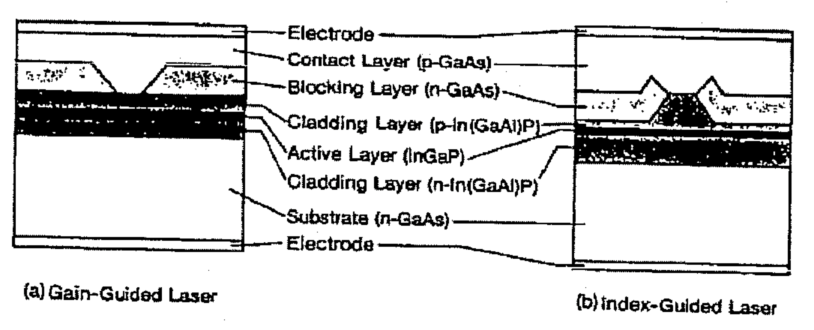
\includegraphics[width=\textwidth]{images/schema.pdf}
    \subcaption{Darstellung des Dioden-Chips.}
    \label{fig:struktur}
  \end{subfigure}
  \caption{Darstellung des Lasers und des Dioden-Chips mit Kennzeichnung der
  Halbeiter-Heterostruktur\cite{anleitung}.}
\end{figure}

Das obere und untere Ende der Dioden wird durch Elektroden abgegrenzt um einen
Anregungsstrom an dem Chip anlegen und ihn somit als Pumpquelle verwenden zu
können. Um einen Resonator zu erzeugen, sind zwei planparallele Schichten
aufgetragen, die vollständig oder teilweise verspiegelt sind. Die anderen
Grenzflächen sind rau, um ungewünschte Oszillationen in weiteren Schichten der
Diode zu verhindern. Abgegrenzt zwischen den Elektroden und einer aktiven Schicht
liegen verschiedene p- und n- dotierte Schichten. Durch ansetzten des
Anregungsstroms wird eine Besetzungsinversion hervorgerufen. In der aktiven
Schicht kommt es zu Elektron-Loch-Rekombinationen, welche Energie (abhängig von der
Bandlücke) in Form von Photonen emittieren. Dieser Vorgang ist in Abbildung
\ref{fig:recombition} graphisch dargestellt.
\begin{figure}[htb]
  \centering
  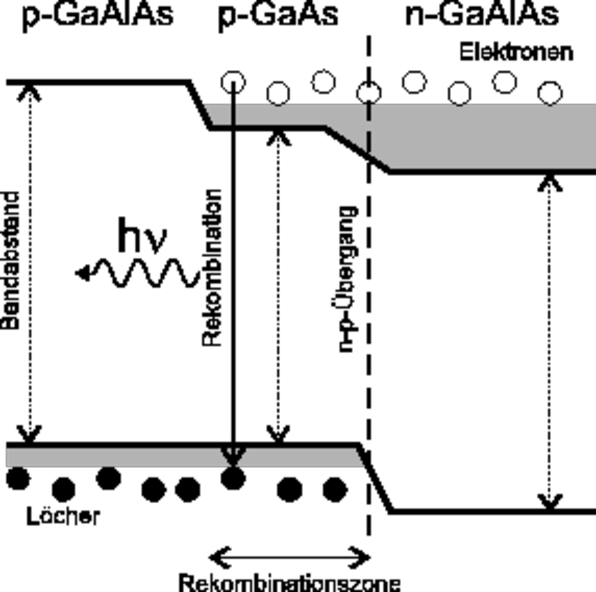
\includegraphics[width=0.5\textwidth]{images/recombition.pdf}
  \caption{Graphische Darstellung der Rekobination eines Elektron-Loch-Paares mit
  emmitiertem Energiequant, ausgehend von der Bandlücken der einzelnen dotierten
  Schichten innerhalb der Laserdiode \cite{recomb}.}
  \label{fig:recombition}
\end{figure}

Innerhalb des durch die unterschiedlich
verspiegelten Außenflächen und des höheren Brechungsindezes der aktiven Schicht
abgegrenzten internen Resonators entstehen dort stehende Wellen. Da die Abmessung
der Diode nicht größer ist als die Wellenlänge des emittierten Lichtes, ist der
von der Diode ausgehende Lichtstrahl elliptischund stark divergent. Um diesem
Abhilfe zu schaffen, wird zusätlich noch eine Linse werdendet, um den Strahl zu
kollimieren.
Der in diesem Experiment verwendete Laser emmittiert Licht
mit einer Wellenlänge von \SIrange{775}{800}{\nano\meter} bei \SI{70}{\milli\watt}
\cite{Sanyo}.
Der nun vorhandene Laserstrahl besitzt zwei ungewünschte Eigenschaften. Zum einen
ist die Linienbreite des Strahls sehr groß ($\Delta\nu \approx \SI{50}{\mega\hertz}$)
im Gegensatz zur Untersuchung atomarer Gegebenheiten ($ \approx \SI{5}{\mega\hertz}$).
Zum anderen ist der Strahl sehr empfindlich auf Änderung optischer Begebenheiten,
was ihn sehr instabil macht. Um diese Effekte anzupassen, wird ein äußerer
Resonator verwendet.

\subsubsection{Äußerer Resonator}
In diesem Experiment wird eine Littrow-Konfiguration, wie in Abbildung \ref{Littrow}
zu sehen verwendet.
\begin{figure}[htb]
  \centering
  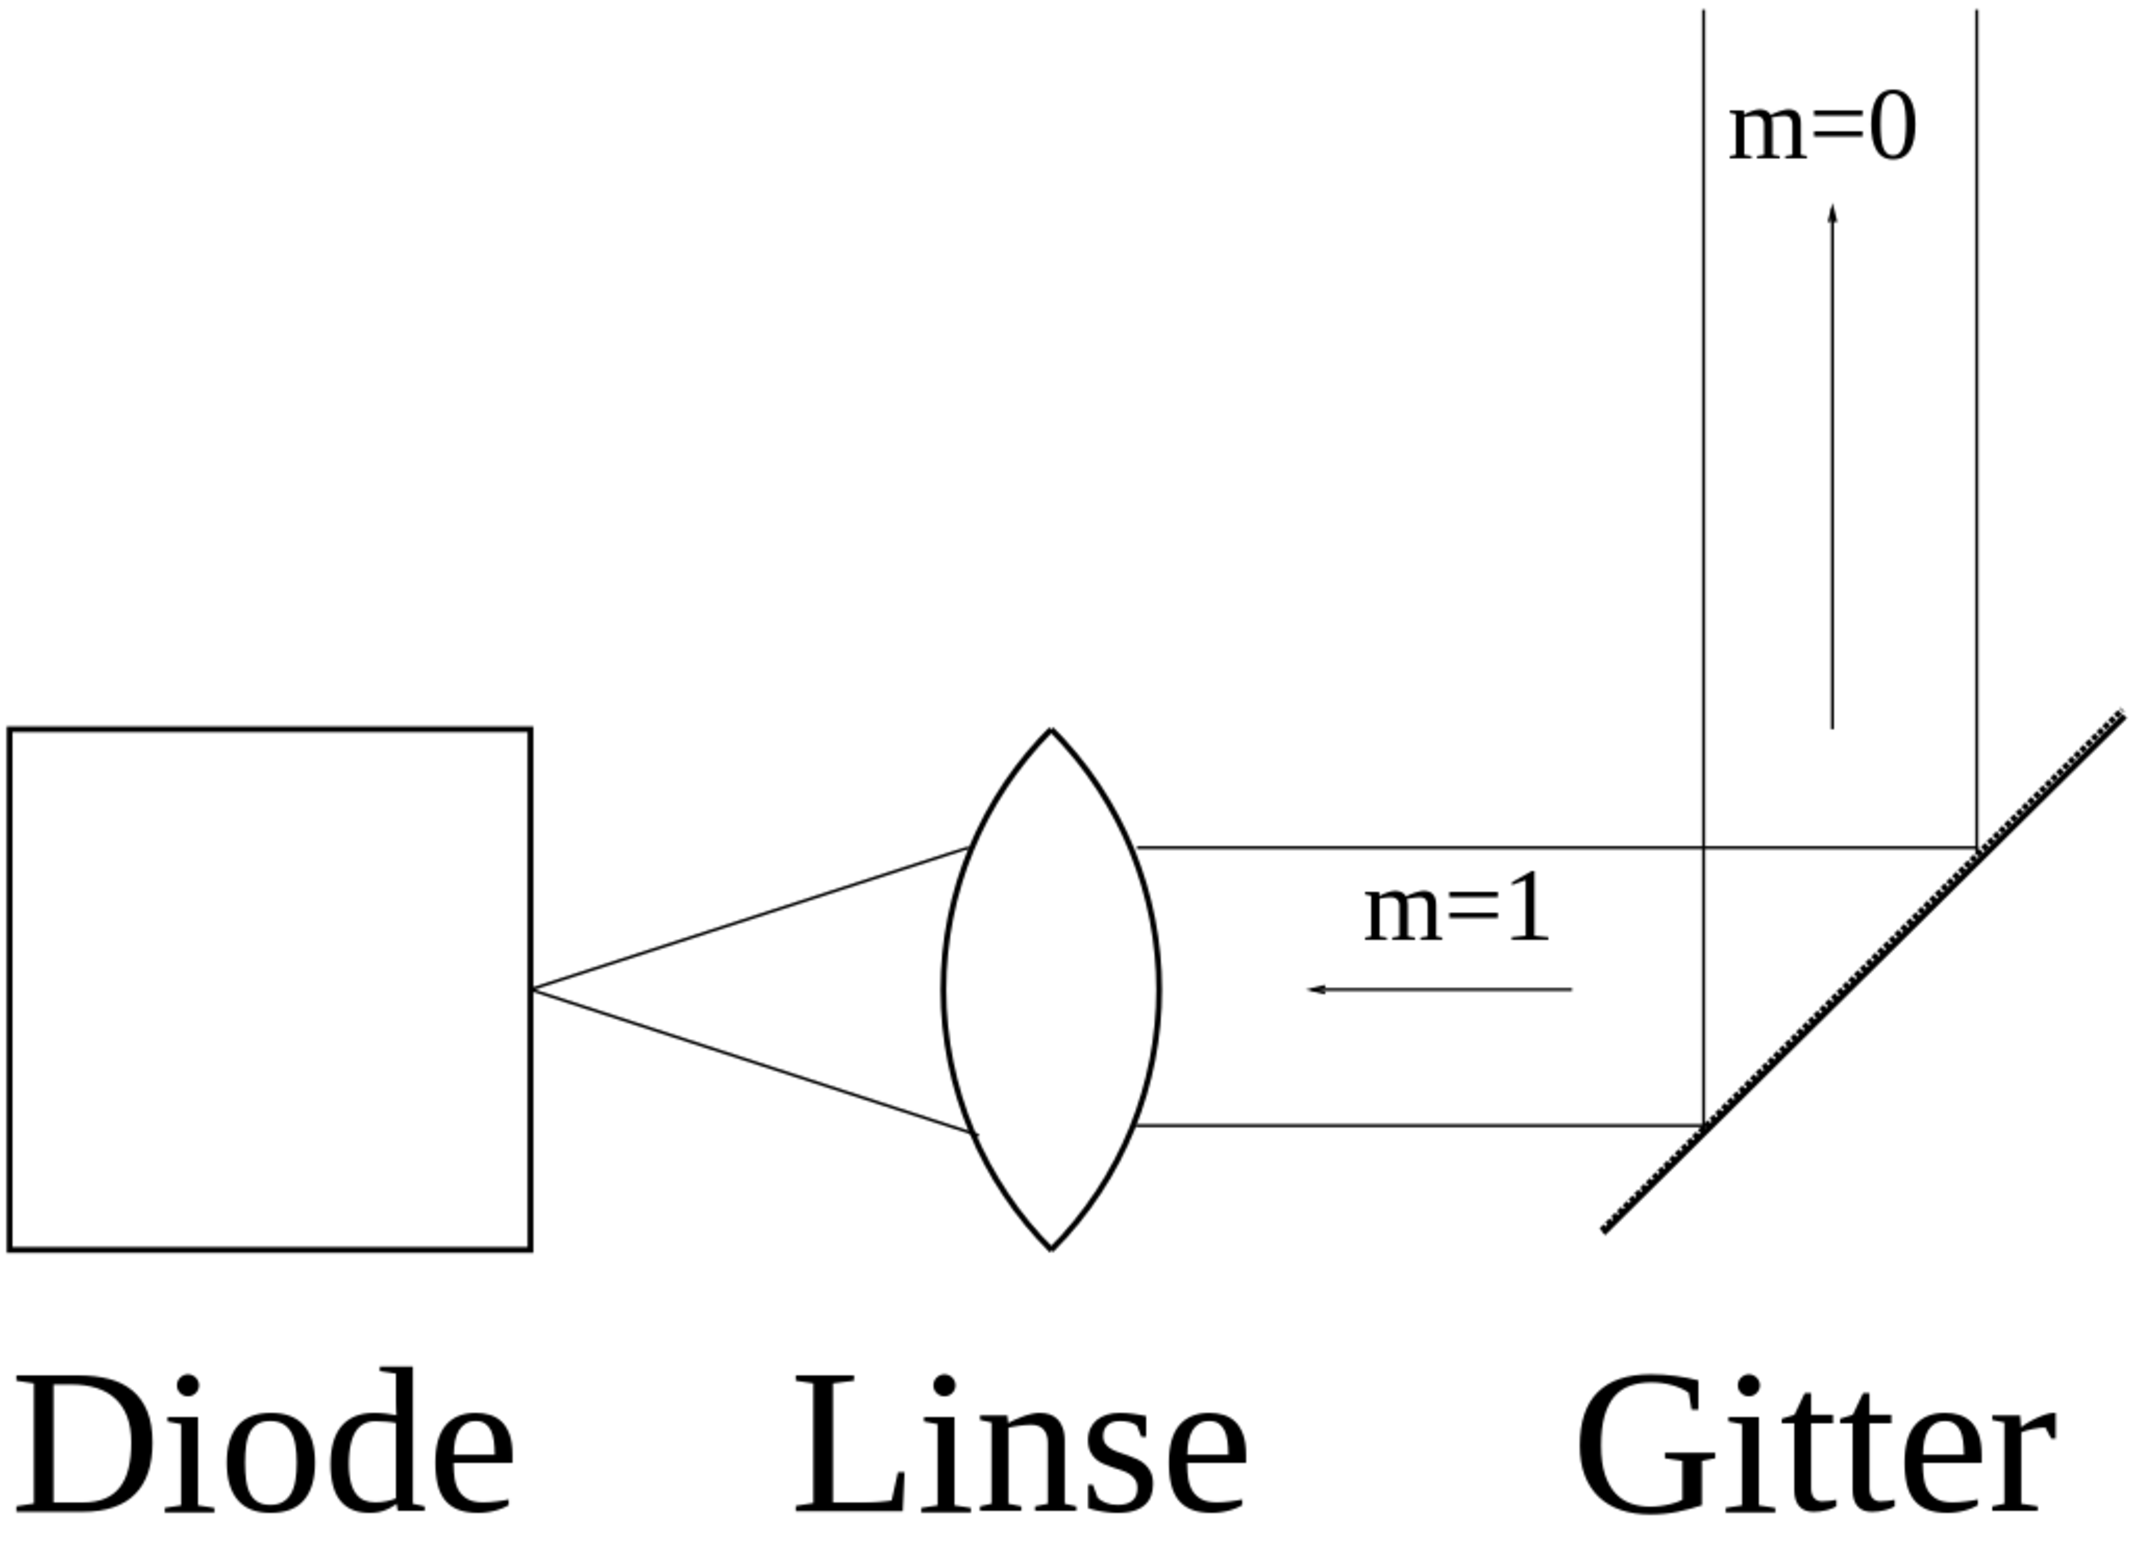
\includegraphics[width=0.5\textwidth]{images/Littrow-Konfig.pdf}
  \caption{Graphische Darstellung einer Littrow-Konfiguration \cite{Littrow-Konfig}.}
  \label{Littrow}
\end{figure}

Dabei wird der äußere Resonator durch eine Linse (Collimating Lens)
und ein Beugungsgitter (Diffraction Grating) realisiert. Die Linse hat wird
verwendet, um den vom Dioden-Chip ausgehenden, stark divergenten Strahl zu
kollimieren. Das Beugungsgitter ist sowohl horizontal als auch vertikal drehbar,
und bestreht aus \SI{1800}{Linien\per\milli\meter}.
Ein Großteil (\SI{75}{\percent}) der Lichtintensität wird durch das Beugungsgitter
direkt reflektiert ($m=\num{0}$), nur \SI{15}{\percent} werden in den Chip reflektiert
($m=\num{1}$). Dies sorgt für zwar für einen kleinen Leistungsverlust, aber einen
wesentlich stabileren Laserstrahl und einer verringerten Linienbreite auf
$\Delta\nu\approx\SI{1}{\mega\hertz}$.


\subsection{Laser Verstärkung}
Um das von Laser emittierte Licht zu abzustimmen, werden Verstärkungen im
Dioden-Chip durch das aktive Medium, durch den internen Resonator, der Gitterrückstreuung
und des externen Resonators verwendet. Dazu ist in Abbildung \ref{fig:net_gain}
die Wellenlänge in Abhängigkeit der einzelenen Verstärkungsweisen aufgetragen.
\begin{figure}[htb]
  \centering
  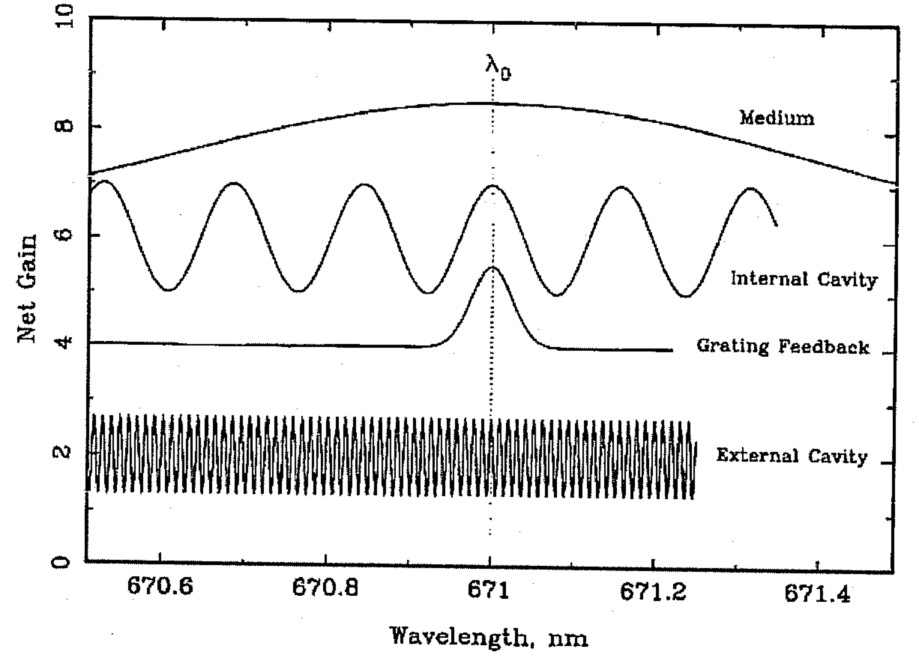
\includegraphics[width=0.7\textwidth]{images/gain-lambda.pdf}
  \caption{Darstellung der Verstärkungen ("Net Gain") gegenüber der Wellenlängen
  \cite{anleitung}.}
  \label{fig:net_gain}
\end{figure}

Das aktive Medium besitzt eine vom Material abhängige Bandlücke. Daraus resultiert
ein breiter Peak in der Wellenlänge \lambda, welcher abhängig von der
Materialtemperatur ist. Um eine Resonanz in der Rubidiumprobe zu erhalten, muss
die Temperatur so eingestellt werden, dass eine Wellenlänge von $\lambda = \SI{780}{\nano\meter}$
erreicht und gehalten wird. Die Abhängigkeit dieser beiden Größen ist in Abbildung
\ref{fig:temp_lambda} dargestellt. Die durchgezogenen Linien repräsentieren hier
die verschiedenen Lasermoden.

Der interne Resonator, abgegrenzt durch zwei reflektierenden Schichten, formt ein
Fabr-Perot-Etalon. Dies ist ein optischer Resonator, bei dem viele kohärente Strahlen
aus dem einfallenden Licht resultieren, indem der Lichtstarhl zwischen den
Abgrenzungen des aktiven Mediums immer wieder reflektiert wird und somit eine
Vielstrahlinterferenz hoher Inferferenzordnung entsteht. Die im Lichtspektrum
entstehende Freuenzänderung $\Delta\nu$ hängt von der Lichtgeschwindigeit $c$,
sowie antiproportional von der Resonatorlänge $L$ und dem Brechungsindex $n$ ab:
\begin{equation}
  \Delta\nu_\text{FSR} = \frac{c}{2Ln}
\end{equation}
Zudem ist die Wellenlänge des Lichts im internen Resonator auf zwei Arten abhängig
vom anliegenden Anregungsstrom. Zum einen wird die Diode von de anlilegenden Strom
erwärmt, was wieder auf das ative Medium wirkt. Zum anderen wird durch den Anregungsstrom
die Ladungsträgerdichte im aktiven Medium und damit der Brechungsindex beeinflusst.
Damit resultiert eine Änderung der Wellenlänge, die in Abbildung \ref{fig:strom_lambda}
zu erkennen ist.

\begin{figure}[htb]
  \begin{subfigure}[c]{0.5\textwidth}
    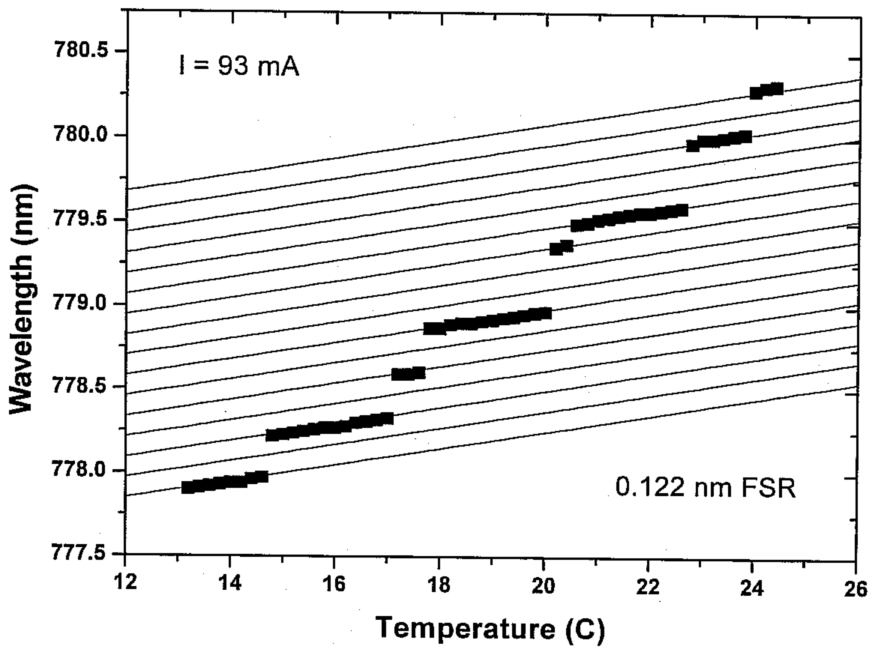
\includegraphics[width=\textwidth]{images/temp-lambda.pdf}
    \subcaption{Abhängigkeiten: Wellenlänge, Temperatur}
    \label{fig:temp_lambda}
  \end{subfigure}
  \begin{subfigure}[c]{0.5\textwidth}
    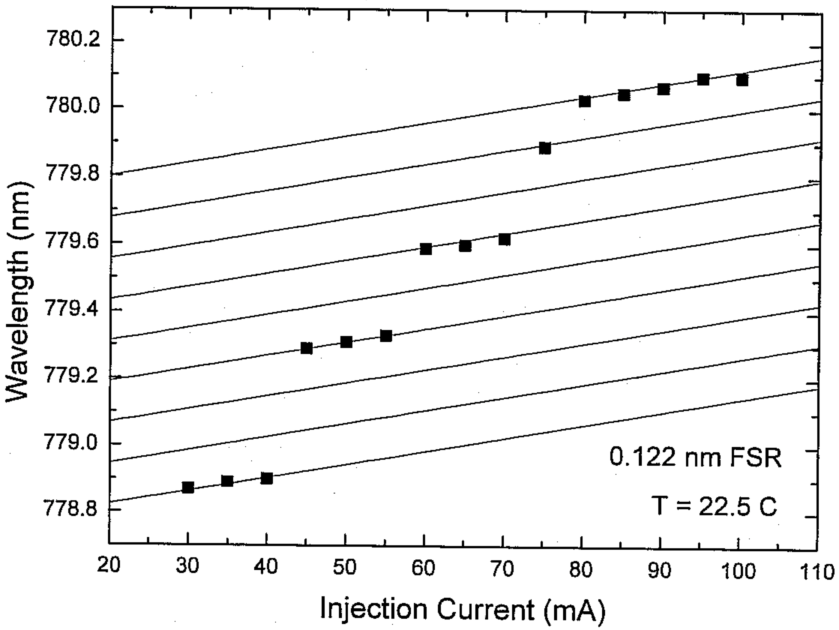
\includegraphics[width=\textwidth]{images/strom-lambda.pdf}
    \subcaption{Abhängigkeit: Wellenlänge, Anregungsstroms}
    \label{fig:strom_lambda}
  \end{subfigure}
  \caption{Abhängigkeitender Wellenlänge von der Temperatur des aktiven Mediums,
  sowie dem angelegten Anregungsstrom \cite{anleitung}.}
\end{figure}

Durch das Beugungsgitter des äußeren Resonators wird nur ein Peak mit Breite
\begin{equation}
  \Delta\nu_{\text{Gitter}} = \frac{\nu}{N}
\end{equation}
der nullten Beugungsordnung ($m=\num{0}$) verwendet, wobei $\nu$ die Frequenz
und $N$ die Gitterzahl darstellt. Um das Licht aus dem Intensitätsmaxima 1.Ordnung
zurück in den Laser zu streuen, kann der horizontale Winkel \theta des Beugungsgitters
manuell verstellt werden. Hier ergibt sich nun nach der Bragg-Bedingung eine
Wellenlänge von
\begin{equation}
    \lambda = 2d\sin{\theta}
\end{equation}
mit der Gitterkonstanten $d$. Wird nun der Anregungsstrom, die temperatur und die
Position des Gitters optimal eingestellt, so ist ein Einmodenbetrieb möglich.


In Abbildung \ref{fig:gain_freq} ist die Verstärkung des Lichtes durch den internen
Resonator, sowie durch den äußeren Resonator und die Gitterrückstreuung gegen
die Frequenz aufgetragen. Bei Veränderung des Winkels am Beugungsgitter verschiebt
sich das Maximum des externen Resonators und es kommt zu einem Modensprung, je
nachdem, welche Mode die höchste Verstärkung erfährt.

\begin{figure}[htb]
  \centering
  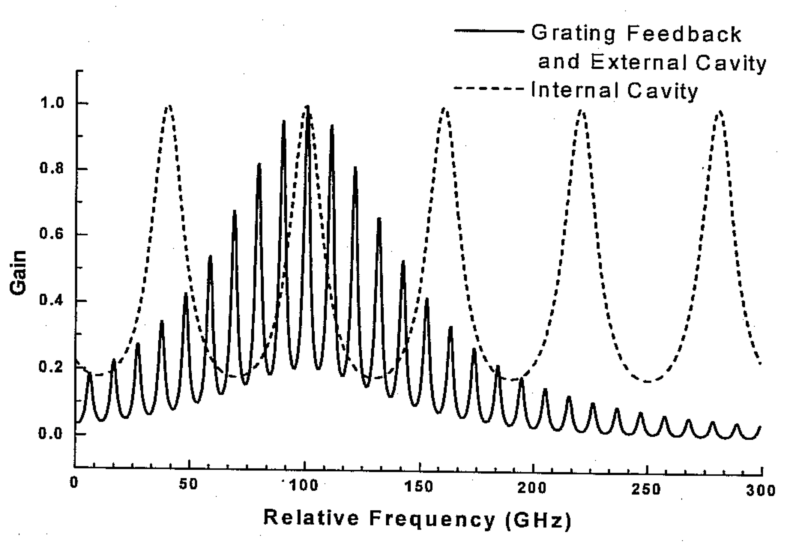
\includegraphics[width=0.7\textwidth]{images/gain-freq.pdf}
  \caption{Aufzeichnung der Lichtverstärkung gegen die Frequenz für den internen
  Resonator und den externen Resonator mit Gitterrückstreuung \cite{anleitung}.}
  \label{fig:gain_freq}
\end{figure}

\subsection{Rubidium Absorptionsspektrum}
Wenn der Lasers bei einer Wellenlänge von $\lambda = \SI{780}{\nano\meter}$ in
einem gewissen Frequenzbereich Licht emittiert, wird von den
beiden in diesem Experiment betrachteten Rubidiumisotopen ($^{85}$Rb und $^{87}$Rb)
derjenige Lichtanteil absorbiert, welcher gleich der Übergangsenergie des jeweiligen
Isotops passt. Diese Übergänge sind in der Graphik \ref{fig:ueber} dargestellt.

\begin{figure}[htb]
  \centering
  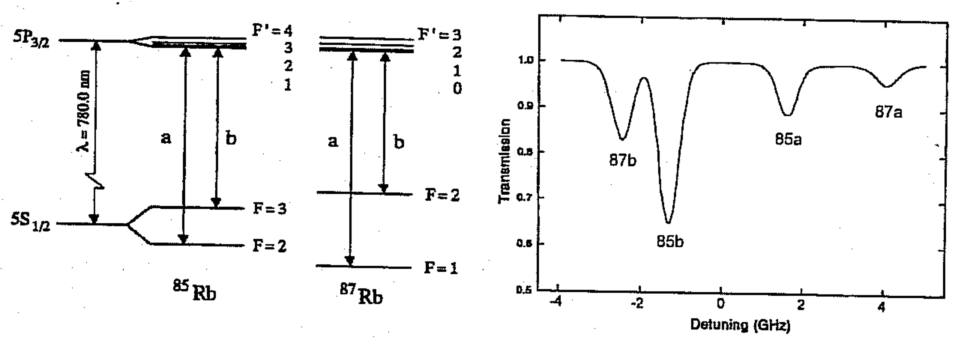
\includegraphics{images/uebergaenge.pdf}
  \caption{Übergänge der Rubidiumisotope $^{85}$Rb und $^{87}$Rb, sowie ein durch
  eine Photodiode aufgenommenes Absorptionsspektrum \cite{anleitung}.}
  \label{fig:ueber}
\end{figure}
